\section{Practical Example}
\label{cha:practical}

This practical example provides a hands-on introduction to the core functionality of Apache Kafka. It demonstrates a simplified scenario to showcase the essential aspects of Kafka's data streaming capabilities. The commands used in this paper apply to Linux; they may differ for other operating systems.

\subsection{Smart Meter}

An EU regulation from the "Clean Energy Package" dictates that 80 \% of households should be equipped with smart meters by 2020. Austrian law requires that 95 \% should be equipped by 2024. Smart meters replace the previous mechanical meters, the Ferraris meters \cite{smartMeterOE}.

The fully electronic smart meters measure energy consumption and power over specific time intervals (e.g. 15 minutes). The measured values are forwarded to the respective grid operators the next day \cite{smartMeterOE}.

A smart meter offers the following new functions: Remote reading by the grid operator, display of consumption values on a display, customer interface, disconnection device and measurement of both energy consumption and energy generation \cite{smartMeterOE}.

\subsubsection{Customer Interface}
All smart meters have a customer interface. With the help of this interface, customers can read detailed consumption and generation information directly from the meter in near real time. The time period in which the data can be read out depends on the manufacturer; in the case of Netz OÖ GmbH's meter, for example, the data is output every second \cite{kernitzkyimehrwert}.

\subsubsection{Smart Meter Adapter}
In Austria, different types of smart meter devices are used by the grid operators. As a result, there are different types of customer interfaces. The Austrian energy industry interest group "Oesterreichs Energie" (\url{https://oesterreichsenergie.at}) has developed a concept for a standardized smart meter adapter that uniforms the provision of data. Therefore it is possible to read the real-time energy data from all smart meters of Austria. The measurement data from this adapter can be queried via MQTT, REST and Modbus TCP. The output format is in JSON and consists of some metadata such as a name defined in the web interface and the measured values with OBIS code and a timestamp \cite{smartMeterAdapter}.

\paragraph{OBIS codes}
The content of the energy measurement data is defined by the IEC 62056-61 standard, which uses a system called OBIS (Object Identification System). The logical OBIS names are represented as a six-character string that corresponds to this OBIS standard. Each data element used in energy meters is uniquely identified by this approach. The complete list of OBIS codes is available on the DLMS Users Association website in the form of a comprehensive Excel file \cite{amaro2011implementing}.

\subsection{Goal}

As more and more IoT (Internet of Things) devices are being used, the amount of data they generate is growing rapidly. In this example, a smart meter adapter is used, but the same ideas can be applied to any IoT device.

To get the data from the smart meter adapter, a local device needs to connect to it via an MQTT broker. This local device could be a Raspberry Pi or another computer running JVM (Java Virtual Machine), MQTT and Kafka. The local device must be connected to the same MQTT broker to which the smart meter adapter is connected, and it must also subscribe to the specific topic to which the smart meter adapter sends its data. In this case, the MQTT broker is also served by the local device.

For a large-scale application, it may not be sufficient to use MQTT alone, so additional streaming functionality is required. The measured values of the smart meter should therefore be streamed via Kafka. In addition to the local device, a Kafka server is needed to process the data and store it for further use. Finally, the energy data can be shared between different services and applications. An illustrative use case could be the forwarding of the data to an energy service provider or the visualization of the data in a mobile app. 

\subsection{Setup MQTT}

First of all, the MQTT broker must be set up on the local device. In this example, Eclipse Mosquitto \cite{mosquitto} was used as the open source MQTT broker.

\subsubsection{Install Eclipse Mosquitto} The following command can be used to install Mosquitto for Debian-based systems:

\begin{lstlisting}[language=bash]
$ sudo apt-get install mosquitto
\end{lstlisting}

\subsubsection{Create config file} The MQTT broker requires a configuration file in order to start properly. This file specifies that it should start with default MQTT port 1883 and allow anonymous access. Mosquitto also supports authentication with username and password, but this is not necessary in this case \cite{mosquitto}. The configuration file named \lstinline{mosquitto.conf} looks like this:

\begin{lstlisting}
listener 1883
allow_anonymous true
\end{lstlisting}

\subsubsection{Start MQTT broker} In Mosquitto, the configuration file can be specified with the \lstinline{-c} option. Therefore, the broker is started with the following command:

\begin{lstlisting}[language=bash]
$ mosquitto -c mosquitto.conf
\end{lstlisting}

\subsection{Connect Smart Meter Adapter}

After starting the broker, the smart meter adapter must send its data to a specific topic. As shown in Figure \ref{fig:sma}, several parameters must be entered. Firstly, the protocol must be determined. As the configured broker does not support encrypted connections, \lstinline{TCP-mqtt} is used. The host name of the local device must be entered in the Broker field, in this case \lstinline{192.168.68.31}. As specified in the configuration file, port 1883 is intended for the broker. In addition, a unique client ID is required for MQTT, which ensures a unique assignment to a specific broker. Redundancies are irrelevant, as the system automatically assigns a new ID in such cases. Finally, a topic must be specified in order to subscribe to it later. Specifically, a simple theme called \lstinline{sma} was used.

\begin{figure}[ht]
    \centering
    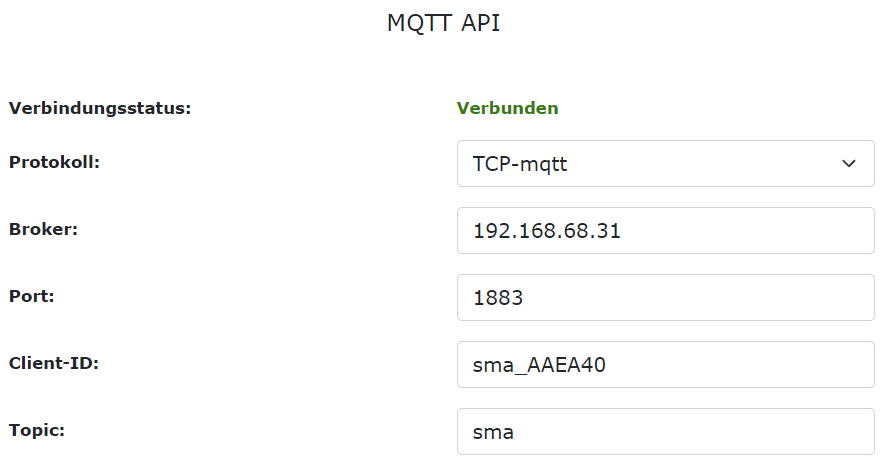
\includegraphics[width=8.5cm]{images/sma.png}
    \caption{MQTT settings of the Smart Meter Adapter.}
    \label{fig:sma}
\end{figure}

\subsection{Setup Kafka}

For demonstration purposes, the local device hosts the Kafka server. In a real-world deployment, however, the Kafka server would be deployed on a remote server or even in a cluster of servers to handle the high volume of data from a large number of smart meters. This enables the application to scale effectively to support a vast network of smart meters.

\subsubsection{Download Apache Kafka} Kafka is available for download in different versions on the official Apache Kafka website: \url{https://kafka.apache.org/downloads}. Once the desired version has been selected, the archive must be downloaded and then unpacked in a suitable location on the system. If the Kafka directory is not contained in the system's PATH environment variable, the following setup commands in this section must be executed within the unpacked Kafka directory.

\subsubsection{Generate a Cluster UUID (Universally Unique ID)} The cluster ID serves as a unique identifier for a Kafka cluster, enabling all nodes within that cluster to recognize each other and collaborate effectively by sharing consistent data and configurations. In this case, a random ID is created, but if there are several instances in the cluster, they must share this ID \cite{shapira2021kafka}. The generation of the ID works as follows:

\begin{lstlisting}[language=bash]
$ KAFKA_CLUSTER_ID=\\
    "$(bin/kafka-storage.sh random-uuid)"
\end{lstlisting}

\subsubsection{Format Log Directories} To ensure proper initialization and readiness of the Kafka data directories for storing new data, it is essential to format the entire data directory, i.e. to capture all partitions, replicas and associated data structures. This comprehensive formatting procedure also deletes all existing data and allows the cluster to reboot, avoiding potential complications due to corrupted or outdated data \cite{shapira2021kafka}. The configuration of the Kafka cluster remains unchanged from the default settings. The formatting process can be performed with the following command:

\begin{lstlisting}[language=bash]
$ bin/kafka-storage.sh format \\
    -t $KAFKA_CLUSTER_ID \\
    -c config/kraft/server.properties
\end{lstlisting}

\subsubsection{Start the Kafka Server} After setting up the cluster, it must be started with KRaft as specified in the next command:

\begin{lstlisting}[language=bash]
$ bin/kafka-server-start.sh \\
    config/kraft/server.properties
\end{lstlisting}

\subsection{Implementation}

With the completion of the initial setup procedures, it is now possible to proceed to the implementation phase of the project. The implementation details of this project are publicly available on GitHub at \url{https://github.com/tformatix/saap-apache-kafka}.

The system is based on a producer-consumer architecture, with the producer running on the local device to collect energy data and the consumer running on another device, e.g. a mobile app, to visualize the data.

\subsubsection{Kafka Producer}

Locally, the \lstinline{SmaMqttConsumer} first subscribes to the MQTT topic \lstinline{sma}, in which the smart meter adapter publishes its measurements. After receiving a measurement, the received JSON is converted into a Kotlin object and forwarded to the \lstinline{SmaKafkaProducer}.

\paragraph{SmaMqttConsumer}

The MQTT consumer uses the package \lstinline{org.eclipse.paho.client.mqttv3}. As MQTT is not the main focus of this paper, it will not be explained further.

\paragraph{SmaKafkaProducer}

The code for the producer class is shown in Figure \ref{fig:producer}. When the class is initialized, a Kafka producer object is created with its properties. These properties include the bootstrap servers, i.e. the initial hosts that the Kafka client uses to find other servers in the cluster \cite{kafkaDoc}. In this example, only one server is running locally, so the bootstrap servers are set to \lstinline{localhost:9092}. Kafka can transmit more than just simple strings, but other objects must be serialized before they can be sent. The serializer and deserializer are responsible for converting objects from one format to another. In this case, the key is simply the name entered in the adapter's web interface and the value is the entire JSON payload. Therefore, only one \lstinline{StringSerializer} is needed.

The \lstinline{produce} method sends a new event to the Kafka stream. A \lstinline{ProducerRecord} object is created that specifies the topic (in this case \lstinline{sma-kafka}) as well as the key and value for the event. Finally, the record is sent to the Kafka cluster.

\begin{figure}[ht]
    \centering
    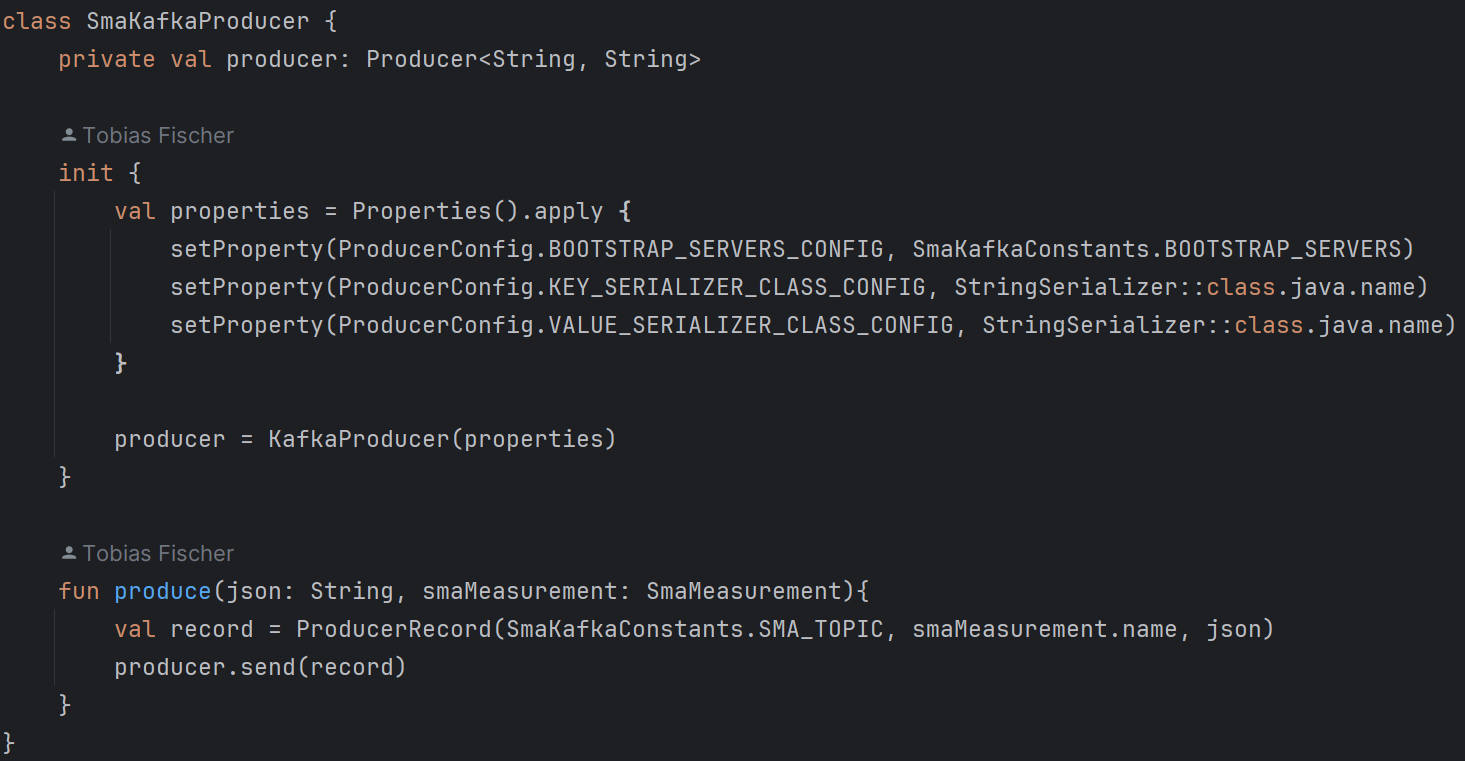
\includegraphics[width=8.5cm]{images/producer.png}
    \caption{SmaKafkaProducer without imports.}
    \label{fig:producer}
\end{figure}

\subsubsection{Kafka Consumer}

In addition to the producer, the \lstinline{SmaKafkaConsumer} class requires two other properties: a group ID and an offset. The implementation of the class can be seen in Figure \ref{fig:consumer}.

Kafka groups consumers in order to distribute the processing load evenly. One or more partitions are assigned to each consumer so that it can concentrate on specific message streams. Within a group, the partitions are distributed among the consumers to avoid overloading a single instance \cite{shapira2021kafka}. In this example, the group ID is generated randomly as there is only one consumer.

The configuration for resetting the automatic offset determines when Kafka starts reading events from the topic. There are two options available: \lstinline{earliest}, which instructs Kafka to start at the beginning of the event stream, and \lstinline{latest}, which restricts Kafka to only process new events \cite{kafkaDoc}. In this case, the \lstinline{earliest} option is used.

The \lstinline{seekToBeginning} method ensures that Kafka retrieves all previously stored events before the consumer starts \cite{kafkaDoc}. The consumer then subscribes to the \lstinline{sma-kafka} topic and enters an infinite loop. Within the loop, the consumer polls for events for one second and then runs through all data records recorded during this time interval.

\begin{figure}[ht]
    \centering
    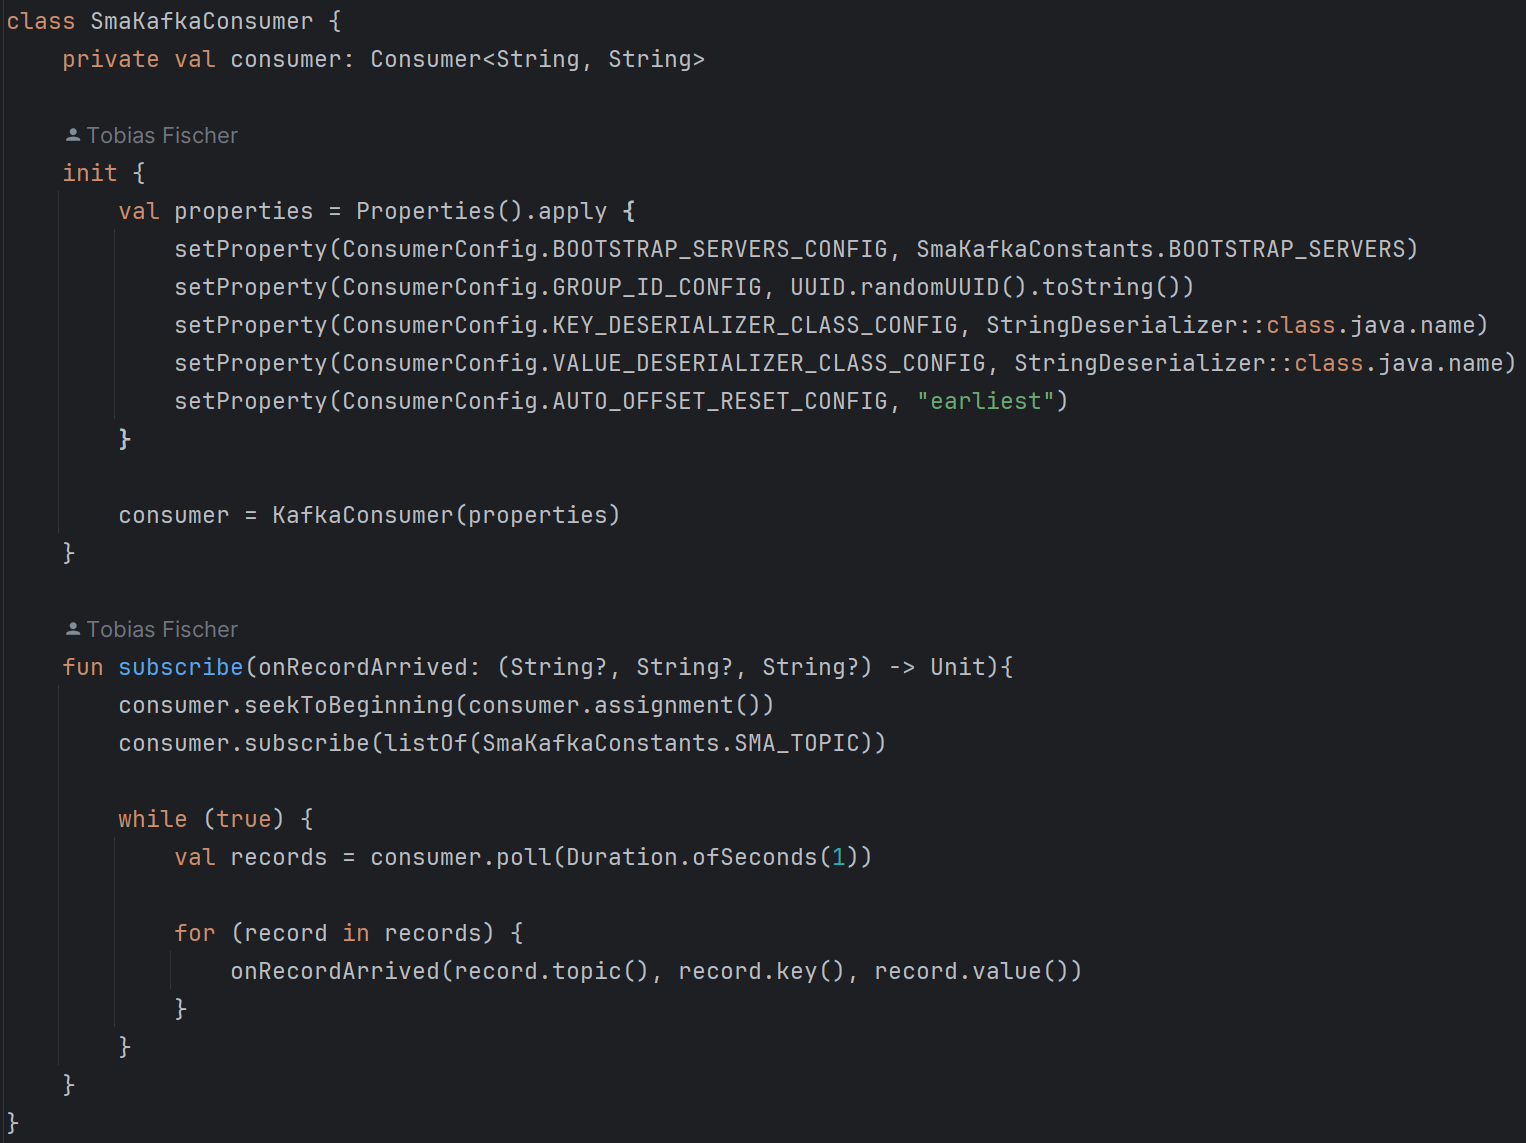
\includegraphics[width=8.5cm]{images/consumer.png}
    \caption{SmaKafkaConsumer without imports.}
    \label{fig:consumer}
\end{figure}
